% !TEX root = ../presentation.tex
% Neural Networks

\begin{slide}{Neural Networks}
  \begin{tikzpicture}[thick]

    % An observation about the world (feature)
    \only<2-3> {
      \path (0, 0)
          coordinate [draw, circle, inner sep=9pt] (x0)
          node {\LARGE$x$};
    }

    % A truth we wish to extract from that observation (output)
    \only<3> {
      \path (4, 0)
            coordinate [draw, circle, inner sep=9pt] (y0)
            node {\LARGE$y$};
      \draw [->] (x0) -- (y0);
    }

    % It's a multi-faceted world (more inputs)
    \only<4-> {
      \path (0, 0)
            coordinate [draw, circle, inner sep=9pt] (x0)
            node {\LARGE$x_{\mathsmaller{0}}$};
      \path (0, 2)
            coordinate [draw, circle, inner sep=9pt] (x1)
            node {\LARGE$x_\mathsmaller{1}$};
    }

    % Reposition
    \only<4-5> {
      \path (4, 1)
            coordinate [draw, circle, inner sep=9pt] (y0)
            node {\LARGE$y$};
      \draw [->] (x0) -- (y0);
      \draw [->] (x1) -- (y0);
    }

    % Some observations are more equal than others
    \only<5> {
      \path (x1) -- (y0) node [midway, above, sloped] {\LARGE $w_1$};
      \path (x0) -- (y0) node [midway, below, sloped] {\LARGE $w_0$};
    }

    % More than one side to a story (more outputs)
    \only<6-> {
      \path (4, 0)
            coordinate [draw, circle, inner sep=9pt] (y0)
            node {\LARGE$y_\mathsmaller{0}$};
      \path (4, 2)
            coordinate [draw, circle, inner sep=9pt] (y1)
            node {\LARGE$y_\mathsmaller{1}$};
      \draw [->] (x0) -- (y1)
            node [pos=0.65, above, sloped] {\LARGE $w_{0, 1}$};
      \draw [->] (x1) -- (y1)
            node [midway, above, sloped] {\LARGE $w_{1, 1}$};
      \draw [->] (x0) -- (y0)
            node [midway, below, sloped] {\LARGE $w_{0, 0}$};
      \draw [->] (x1) -- (y0)
            node [pos=0.65, below, sloped] {\LARGE $w_{1, 0}$};
    }

    % We all have biases
    % \only<7-> {
    %   \path (2.5, 3.5)
    %         coordinate [draw, circle, inner sep=8pt] (b1)
    %         node {\LARGE$b_\mathsmaller{1}$};
    %   \path (2.5, -1.5)
    %         coordinate [draw, circle, inner sep=8pt] (b0)
    %         node {\LARGE$b_\mathsmaller{0}$};
    %
    %   \draw [->] (b0) -- (y0);
    %   \draw [->] (b1) -- (y1);
    % }

    % It turns out what we thought was true, really wasn't
    \only<7-> {
    \path (5.25, 1) coordinate node {\Huge$\leadsto$};
    \path (6.5, 1)
          coordinate [draw, circle, inner sep=9pt] (hat)
          node {\LARGE$\hat{y}$};
    }
  \end{tikzpicture}

  \only<8> {
    $$
    \begin{sbmatrix}{\mathbf{x}}
      x_0 & x_1
    \end{sbmatrix}
    \times
    \begin{sbmatrix}{\mathbf{W}}
      w_{0, 0} & w_{0, 1} \\
      w_{1, 0} & w_{1, 1}
    \end{sbmatrix}
    +
    \begin{sbmatrix}{\mathbf{b}}
      b_0 \\
      b_1
    \end{sbmatrix}
    =
    \begin{sbmatrix}{\mathbf{y}}
      y_0 \\
      y_1
    \end{sbmatrix}
    $$
  }

  \only<9> {
    $$
    \begin{sbmatrix}{\mathbf{x}}
      x_0 & x_1
    \end{sbmatrix}
    \times
    \begin{sbmatrix}{\mathbf{W}}
      w_{0, 0} & w_{0, 1} \\
      w_{1, 0} & w_{1, 1}
    \end{sbmatrix}
    +
    \begin{sbmatrix}{\mathbf{b}}
      b_0 \\
      b_1
    \end{sbmatrix}
    =
    \begin{sbmatrix}{\mathbf{y}}
      y_0 \\
      y_1
    \end{sbmatrix}
    \hspace{0.2cm}\leadsto\hspace{0.2cm}
    \textcolor{black}{\hat{\mathbf{y}}}
    $$
  }
\end{slide}

\begin{slide}{Neural Networks}
  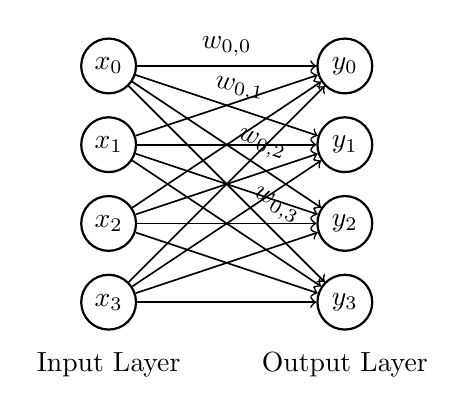
\begin{tikzpicture}
    % Input layer
    \foreach \i in {0, ..., 3} {
      \path (0, {-\i}) coordinate [draw, circle, thick, inner sep=7pt]
            (x\i) node {$x_\i$};
    }
    \path (0, -3.8) node {Input Layer};

    % Output layer
    \foreach \i in {0, ..., 3} {
      \path (3, {-\i}) coordinate [draw, circle, thick, inner sep=7pt]
            (y\i) node {$y_\i$};
    }
    \path (3, -3.8) node {Output Layer};

    % Connections
    \onslide<2->{
      \foreach \i in {0, ..., 3} {
        \foreach \j in {0, ..., 3} {
          \ifnum\i=0
            \draw [semithick, ->] (x\i) -- (y\j);
          \else
            \onslide<4-> {
              \draw [semithick, ->] (x\i) -- (y\j);
            }
          \fi
        }
        \ifnum\i=0
          \onslide<3>{
            \draw [line width=0] (x0) -- (y0)
                  node [above, midway] {$w_{0,0}$};

            \draw [line width=0] (x0) -- (y1)
                  node [above, pos=0.55, rotate=-10] {$w_{0,1}$};

            \draw [line width=0] (x0) -- (y2)
                  node [above, pos=0.65, rotate=-20] {$w_{0,2}$};

            \draw [line width=0] (x0) -- (y3)
                  node [above, pos=0.7, rotate=-30] {$w_{0,3}$};
          }
        \fi
      }
    }
  \end{tikzpicture}
\end{slide}

\begin{slide}{Deep Neural Networks}
  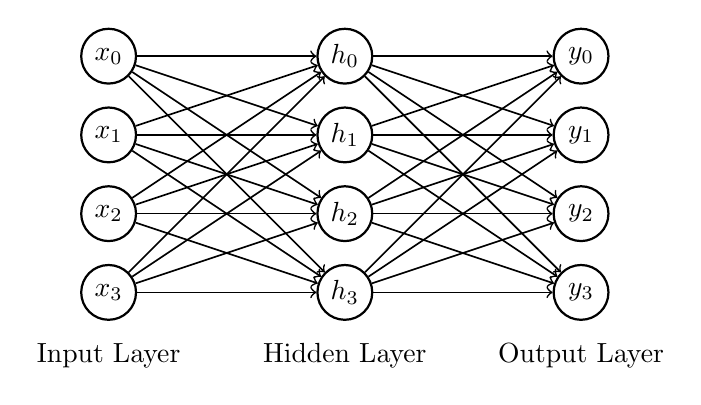
\begin{tikzpicture}
    % Input layer
    \foreach \i in {0, ..., 3} {
      \path (0, {-\i}) coordinate [draw, circle, thick, inner sep=7pt]
            (x\i) node {$x_\i$};
    }
    \path (0, -3.8) node {Input Layer};

    % Hidden layer
    \foreach \i in {0, ..., 3} {
      \path (3, {-\i}) coordinate [draw, circle, thick, inner sep=7pt]
            (h\i) node {$h_\i$};
    }
    \path (3, -3.8) node {Hidden Layer};

    % Output layer
    \foreach \i in {0, ..., 3} {
      \path (6, {-\i}) coordinate [draw, circle, thick, inner sep=7pt]
            (y\i) node {$y_\i$};
    }
    \path (6, -3.8) node {Output Layer};

    % Connections
      \foreach \i in {0, ..., 3} {
        \foreach \j in {0, ..., 3} {
            \draw [semithick, ->] (x\i) -- (h\j);
            \draw [semithick, ->] (h\i) -- (y\j);
        }
      }
  \end{tikzpicture}
\end{slide}

\begin{slide}{Deep Neural Networks}
  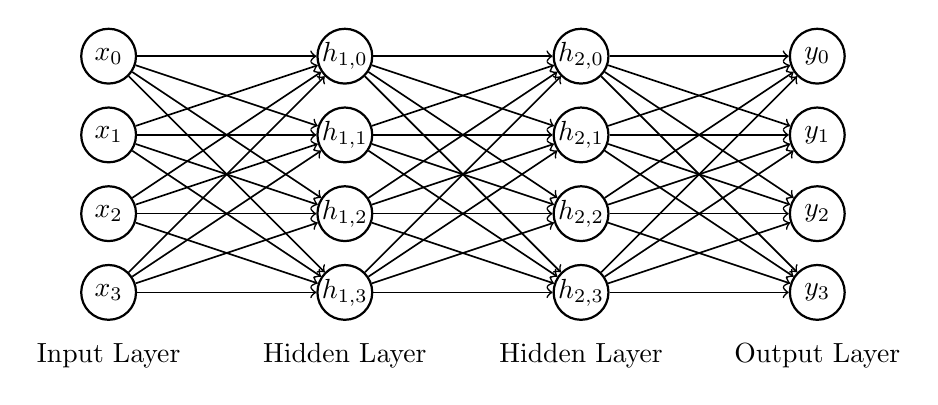
\begin{tikzpicture}
    % Input layer
    \foreach \i in {0, ..., 3} {
      \path (0, {-\i}) coordinate [draw, circle, thick, inner sep=7pt]
            (x\i) node {$x_\i$};
    }
    \path (0, -3.8) node {Input Layer};

    % Hidden layer
    \foreach \i in {0, ..., 3} {
      \path (3, {-\i}) coordinate [draw, circle, thick, inner sep=7pt]
            (h1\i) node {$h_{1,\i}$};
    }
    \path (3, -3.8) node {Hidden Layer};

    % Hidden layer
    \foreach \i in {0, ..., 3} {
      \path (6, {-\i}) coordinate [draw, circle, thick, inner sep=7pt]
            (h2\i) node {$h_{2,\i}$};
    }
    \path (6, -3.8) node {Hidden Layer};

    % Output layer
    \foreach \i in {0, ..., 3} {
      \path (9, {-\i}) coordinate [draw, circle, thick, inner sep=7pt]
            (y\i) node {$y_\i$};
    }
    \path (9, -3.8) node {Output Layer};

    % Connections
      \foreach \i in {0, ..., 3} {
        \foreach \j in {0, ..., 3} {
            \draw [semithick, ->] (x\i) -- (h1\j);
            \draw [semithick, ->] (h1\i) -- (h2\j);
            \draw [semithick, ->] (h2\i) -- (y\j);
        }
      }
  \end{tikzpicture}
\end{slide}

\begin{slide}{Deep Neural Networks}
{\Large
  Deep Learning assumes that data is structured\\

  \onslide<2->{
    \vspace{1cm}
      {\Huge  hierarchically}
  }
}
\end{slide}

\begin{slide}{Deep Neural Networks}
  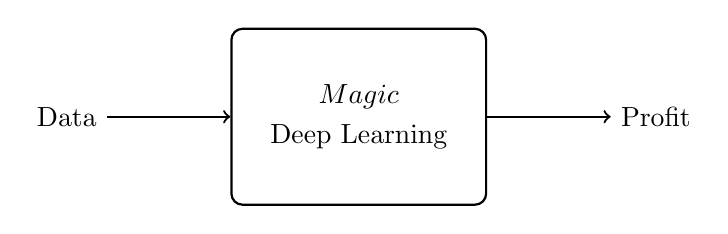
\begin{tikzpicture}[thick]
    \path (0, 0) coordinate
          [draw,
           rectangle,
           rounded corners,
           text width=3cm,
           text height = 2cm] (dl);
    \draw (0, 0.25) node {$\cancel{\text{Magic}}$};
    \draw (0, -0.25) node {Deep Learning};

    \path (-3.2, 0) coordinate (data) node [left] {Data};
    \path (3.2, 0) coordinate (profit) node [right] {Profit};

    \draw [->] (data) -- (dl);
    \draw [->] (dl) -- (profit);
  \end{tikzpicture}
\end{slide}
